\begin{definition}{Réseaux Bayésiens}{bayesianNetworks}
    Un réseau bayésien est un graphe orienté acyclique (DAG) dont les nœuds représentent des variables aléatoires et les arcs représentent des dépendances conditionnelles.\\
    Ils permettent de représenter des distributions de probabilités conjointes de manière compacte, de construire des modèles de raisonnement probabiliste et de faire de l'inférence.
    \begin{itemize}
        \item Les nœuds représentent des variables aléatoires
        \item Les arcs représentent des dépendances (\textit{causilités?}) conditionnelles ainsi que des distributions de probabilités pour chaque variable aléatoire \textbf{étant donné} ses parents
        % \item Les nœuds sont associés à des probabilités conditionnelles
    \end{itemize}
    Façon compacte de représenter des probabilités conjointes.
    
\end{definition}

% \begin{example}\leavevmode
%     \begin{figure}[H]
%         \centering
%         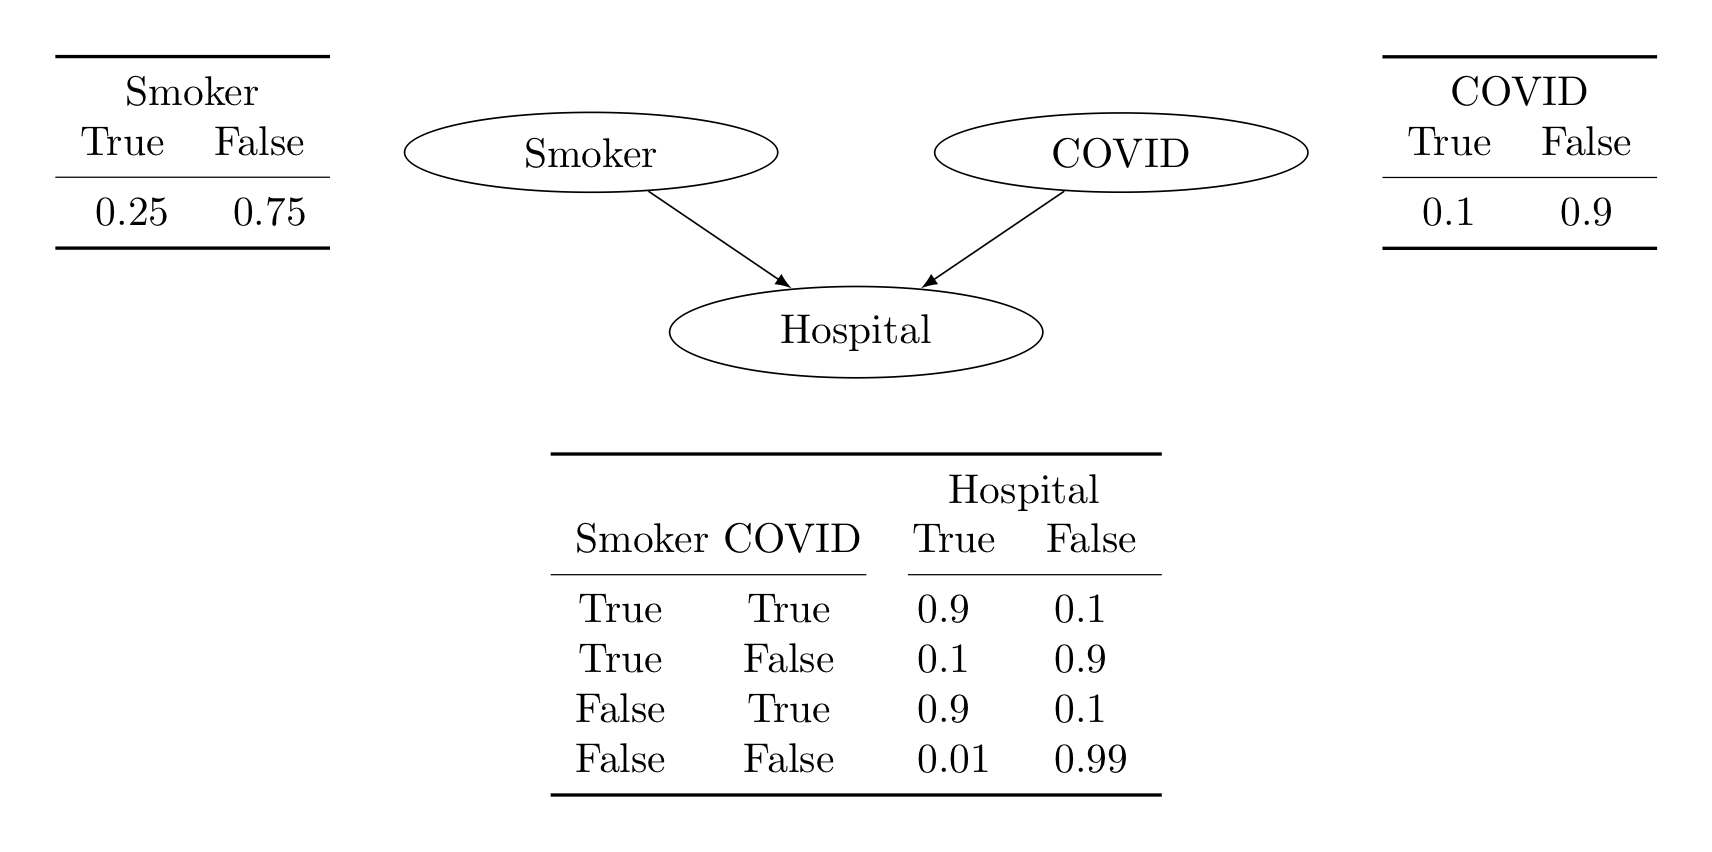
\includegraphics[width=0.6\linewidth]{pictures/bayesianNetwork.png}
%         \caption{Réseau bayésien}
%         \label{fig:bayesianNetwork}
%     \end{figure}
% \end{example}

La topologie du \textbf{RB} modélise les relations de causalités entre les variables aléatoires. 

Un arc $X \rightarrow Y$ signifie que $X$ influence $Y$.

Si $X$ n'a pas de parents, alors sa distribution de probabilité est dite \textbf{inconditionnelle} ou \textbf{à priori}.
Si $X$ a des parents, alors sa distribution de probabilité est dite \textbf{conditionnelle} ou \textbf{à posteriori}.


\begin{example}\leavevmode
    Voici un exemple du livre \textit{Artificial Intelligence: A Modern Approach} de Stuart Russel et Peter Norvig. 
    Considérons la situation suivante: 
    \begin{itemize}
        \item Je suis au travail et mes voisins Marie et John m'ont promis de \textbf{m'appeller} chaque fois que mon \textbf{alarme} se déclenche.
        \item \textbf{Jean m'appelle} pour me dire que mon alarme s'est déclenchée. 
            \begin{itemize}
                \item Cependant, il \textbf{la confond } parfois avec la sonnerie du téléphone
            \end{itemize}
        \item \textbf{Marie m'appelle pas toujours} 
            \begin{itemize}
                \item Elle écoute de la musique et ne l'entend pas toujours
            \end{itemize}
        \item Mon alarme peut également sonner à cause de \textbf{séismes}. 
        \item $\longrightarrow$ \textbf{Comment conclure qu'il y a un cambriolage?}
    \end{itemize}
    On représente cette situation par le réseau bayésien suivant: 
    % construit le graphe avec tikz
    \begin{figure}[H]
    \centering
    \scalebox{0.8}{
        \begin{minipage}{0.45\textwidth}
            \begin{tikzpicture}
              % Dessinez les nœuds du graphe
                \node[state] (0) at (0,0) {Alarme};
                \node[state] (1) [above right =of 0] {Séisme};
                \node[state] (2) [above left =of 0] {Combriolage};
                \node[state] (3) [below right =of 0] {MarieAppelle};
                \node[state] (4) [below left =of 3] {JeanAppelle};
                
                \path (2) edge[arrow] (0);
                % \path (1) edge[arrow][loop above] (1);
                \path (1) edge[arrow] (0);
                \path (0) edge[arrow] (3);
                \path (0) edge[arrow] (4);
            \end{tikzpicture}
            \caption{Réseau bayésien de l'exemple}
            \label{fig:graph1}
        \end{minipage}
    }
    \end{figure}
    Voici les probabilités conditionnelles associées à ce réseau bayésien: 
    \begin{figure}[H]
        \centering
        \scalebox{0.8}{
            \begin{minipage}{0.45\textwidth}
                \begin{tabular}{|c|c|}
                    \hline
                    $P(Combriolage)$ & $P(\neg Combriolage)$ \\
                    \hline
                    0.001 & 0.999 \\
                    \hline
                \end{tabular}
                \caption{Probabilités de $Combriolage$}
                \label{fig:graph1}
            \end{minipage}
            \begin{minipage}{0.45\textwidth}
                \begin{tabular}{|c|c|}
                    \hline
                    $P(Séisme)$ & $P(\neg Séisme)$ \\
                    \hline
                    0.002 & 0.998 \\ 
                    \hline
                \end{tabular}
                \caption{Probabilités de $Séisme$}
                \label{fig:graph1}
            \end{minipage}
        } 

        \scalebox{0.8}{
            \begin{minipage}{0.45\textwidth}
                \begin{tabular}{|c|c|c|}
                    \hline
                    $Combriolage$ & $Séisme$ & $P(Alarme)$ \\
                    \hline
                    $V$ & $V$ & 0.95 \\ 
                    $V$ & $F$ & 0.94 \\ 
                    $F$ & $V$ & 0.29 \\ 
                    $F$ & $F$ & 0.001 \\
                    \hline
                \end{tabular}
                \caption{Probabilités conditionnelles de $Alarme$}
                \label{fig:graph1}
            \end{minipage}
        } 

        \scalebox{0.8}{
            \begin{minipage}{0.45\textwidth}
                \begin{tabular}{|c|c|}
                    \hline
                    $Alarme$ & $P(JeanAppelle)$ \\
                    \hline
                    $V$ & 0.90 \\
                    $F$ & 0.05 \\
                    \hline
                \end{tabular}
                \caption{Probabilités conditionnelles de $JeanAppelle$}
                \label{fig:graph1}
            \end{minipage}
            \begin{minipage}{0.45\textwidth}
                \begin{tabular}{|c|c|}
                    \hline
                    $Alarme$ & $P(MarieAppelle)$ \\
                    \hline
                    $V$ & 0.70 \\
                    $F$ & 0.01 \\
                    \hline
                \end{tabular}
                \caption{Probabilités conditionnelles de $MarieAppelle$}
                \label{fig:graph1}
            \end{minipage}
        } 
    \end{figure}

\end{example}

\begin{note}
    Les réseaux bayésiens peuvent avoir des variables aléatoires continues ou discrètes.
\end{note}

Nous savons que par définition, $P(A,B) = P(A|B)P(B)$.
Nous pouvons donc écrire la probabilité conjointe d'un réseau bayésien comme suit: 
\begin{equation}
    P(X_1, X_2, \dots, X_n) = \prod_{i=1}^{n} P(X_i | Parents(X_i)) 
\end{equation} 
Où $Parents(X_i)$ est l'ensemble des parents directe de $X_i$ dans le réseau bayésien.

\begin{example}\leavevmode
    En utilisant le réseau bayésien de l'exemple précédent, nous pouvons calculer la probabilité conjointe de toutes les variables aléatoires comme suit: 
    \begin{align*}
        P(C=F, S=F, A=V, J=V, M=V) \\ 
        &= P(C=F)P(S=F)P(A=V|C=F, S=F)P(J=V|A=V)P(M=V|A=V) \\
        &= 0.999 \times 0.998 \times 0.001 \times 0.90 \times 0.70 \\
        &= 0.000628
    \end{align*}
\end{example}

Pour calculer les probabilités marginales, on peut ignorer les noeuds 
\textbf{dont les descendants ne sont pas les noeuds observés}

\begin{example}\leavevmode
    \begin{align*}
        P(C=F \cap A=V) &= \sum_{s} \sum_{j} \sum_{m} P(C=F, S=s, A=V, J=j, M=m) \\
                        &= \sum_{s} P(A=V | C=f, s) P(C=F) P(S=s) 
    \end{align*}
    On peut ignorer $J$ et $M$ car ils ne sont pas des descendants de $C$ qui est observé.
    Cependant, on ne peut pas ignorer $S$ car A est un descendant de $S$ et $A$ est observé.
\end{example}
